% !TEX program = xelatex
\documentclass[10pt,letterpaper,twocolumn]{article}

% === GEOMETRY ===
\usepackage[top=0.75in, bottom=0.75in, left=0.75in, right=0.75in]{geometry}

% === FONTS ===
\usepackage{fontspec}
\usepackage{unicode-math}
\usepackage{xeCJK}
\setCJKmainfont{Droid Sans Japanese}

\setmainfont{Latin Modern Roman}
\setsansfont{Latin Modern Sans}

\newfontfamily\acbold{ywft-processing-bold}[
  Path=../../system/public/type/webfonts/,
  Extension=.ttf
]
\newfontfamily\aclight{ywft-processing-light}[
  Path=../../system/public/type/webfonts/,
  Extension=.ttf
]
\newfontfamily\kidlispfont{ComicRelief-Regular}[
  Path=fonts/,
  Extension=.ttf
]
\newfontfamily\kidlispbold{ComicRelief-Bold}[
  Path=fonts/,
  Extension=.ttf
]
\setmonofont{Latin Modern Mono}[Scale=0.85]

% === PACKAGES ===
\usepackage{xcolor}
\usepackage{titlesec}
\usepackage{enumitem}
\usepackage{booktabs}
\usepackage{tabularx}
\usepackage{multicol}
\usepackage{fancyhdr}
\usepackage{hyperref}
\usepackage{graphicx}
\graphicspath{{figures/}}
\usepackage{ragged2e}
\usepackage{listings}
\usepackage{natbib}
\usepackage[colorspec=0.92]{draftwatermark}

% === COLORS (AC palette) ===
\definecolor{acpink}{RGB}{180,72,135}
\definecolor{acpurple}{RGB}{120,80,180}
\definecolor{acdark}{RGB}{64,56,74}
\definecolor{acgray}{RGB}{119,119,119}
\definecolor{klbrand}{RGB}{205,92,155}
\definecolor{klcyan}{RGB}{112,214,255}
\definecolor{kldark}{RGB}{48,43,58}
\definecolor{draftcolor}{RGB}{205,92,155}

% === DRAFT WATERMARK ===
\DraftwatermarkOptions{
  text=WORKING DRAFT,
  fontsize=3cm,
  color=draftcolor!18,
  angle=45,
  pos={0.5\paperwidth, 0.5\paperheight}
}

% === KIDLISP SYNTAX COLORS ===
\definecolor{klfn}{RGB}{0,136,170}
\definecolor{klform}{RGB}{119,51,170}
\definecolor{klrepeat}{RGB}{170,0,170}
\definecolor{klnum}{RGB}{204,0,102}
\definecolor{klstr}{RGB}{170,120,0}
\definecolor{klcmt}{RGB}{102,102,102}
\definecolor{klmath}{RGB}{0,136,0}
\definecolor{klvar}{RGB}{204,102,0}
\definecolor{klembed}{RGB}{0,136,0}

\newcommand{\kn}[1]{\textcolor{klnum}{#1}}
\newcommand{\kt}[1]{\textcolor{klstr}{#1}}
\newcommand{\kv}[1]{\textcolor{klvar}{#1}}
\newcommand{\ke}[1]{\textcolor{klembed}{\textbf{#1}}}
\newcommand{\km}[1]{\textcolor{klmath}{#1}}

% === HYPERREF ===
\hypersetup{
  colorlinks=true,
  linkcolor=acpurple,
  urlcolor=acpurple,
  citecolor=acpurple,
  pdfauthor={@jeffrey},
  pdftitle={KidLisp '26：ジェネラティブアートのためのミニマルLisp},
}

% === SECTION FORMATTING ===
\titleformat{\section}
  {\normalfont\bfseries\normalsize\uppercase}
  {\thesection.}
  {0.5em}
  {}
\titlespacing{\section}{0pt}{1.2em}{0.3em}

\titleformat{\subsection}
  {\normalfont\bfseries\small}
  {\thesubsection}
  {0.5em}
  {}
\titlespacing{\subsection}{0pt}{0.8em}{0.2em}

% === HEADER/FOOTER ===
\pagestyle{fancy}
\fancyhf{}
\renewcommand{\headrulewidth}{0pt}
\fancyhead[C]{\footnotesize\color{acpink}\textit{作業草稿 --- 引用不可}}
\fancyfoot[C]{\footnotesize\thepage}

% === CUSTOM COMMANDS ===
\newcommand{\acdot}{{\color{acpink}.}}
\newcommand{\kidlisp}{\textsc{KidLisp}}

% === LISTINGS ===
\lstdefinelanguage{kidlisp}{
  morekeywords=[1]{wipe,ink,line,box,circle,tri,plot,flood,shape,zoom,scroll,spin,blur,contrast,embed,layer,width,height,frame,time,wiggle,melody,mic,suck,sort,form,trans,cube,move,scale,hop,overtone,resolution,write,text,type,stamp,paste,point,poly,noise,fade,pan,unpan,mask,unmask,flip},
  morekeywords=[2]{def,let,if,cond,once,later,lambda,do},
  morekeywords=[3]{repeat},
  morekeywords=[4]{random,sin,cos,tan,floor,ceil,round,abs,sqrt,min,max},
  sensitive=true,
  morecomment=[l]{;},
  morestring=[b]",
  escapeinside={|}{|},
}
\lstset{
  language=kidlisp,
  basicstyle=\ttfamily\small,
  keywordstyle=[1]\color{klfn}\bfseries,
  keywordstyle=[2]\color{klform}\bfseries,
  keywordstyle=[3]\color{klrepeat}\bfseries,
  keywordstyle=[4]\color{klmath},
  commentstyle=\color{klcmt}\itshape,
  stringstyle=\color{klstr},
  breaklines=true,
  frame=single,
  rulecolor=\color{acgray!30},
  backgroundcolor=\color{acgray!5},
  xleftmargin=0.5em,
  xrightmargin=0.5em,
  aboveskip=0.5em,
  belowskip=0.5em,
}

\lstdefinelanguage{json}{
  basicstyle=\ttfamily\small,
  stringstyle=\color{acpink},
  morestring=[b]",
  literate=
    {:}{{{\color{acgray}:}}}{1}
    {,}{{{\color{acgray},}}}{1}
    {\{}{{{\color{acgray}\{}}}{1}
    {\}}{{{\color{acgray}\}}}}{1},
}

% === LIST SETTINGS ===
\setlist[itemize]{nosep, leftmargin=1.2em, itemsep=0.1em}
\setlist[enumerate]{nosep, leftmargin=1.2em}

\setlength{\columnsep}{1.8em}
\setlength{\parindent}{1em}
\setlength{\parskip}{0.3em}

% Hyphenation for narrow two-column layout
\tolerance=800
\emergencystretch=1em
\hyphenpenalty=50

\begin{document}

\twocolumn[{%
\begin{center}

\includegraphics[height=4em]{pals}\par\vspace{0.5em}
{\kidlispbold\fontsize{26pt}{30pt}\selectfont\color{kldark} Kid{\color{klbrand}Lisp} '26}\par
\vspace{0.2em}
{\kidlispfont\fontsize{11pt}{13pt}\selectfont\color{klbrand} ジェネラティブアートのためのミニマルLisp}\par
\vspace{0.6em}
{\normalsize @jeffrey}\par
{\small\color{acgray} Aesthetic.Computer}\par
{\small\color{acgray} ORCID: \href{https://orcid.org/0009-0007-4460-4913}{0009-0007-4460-4913}}\par
\vspace{0.3em}
{\small\color{acpurple} \url{https://kidlisp.com} \enspace$\cdot$\enspace \url{https://aesthetic.computer}}\par
\vspace{0.6em}
\rule{\textwidth}{1.5pt}
\vspace{0.5em}
\end{center}

\begin{center}
{\small\color{acpink}\textbf{[ 作業草稿 --- 引用不可 ]}}
\end{center}
\vspace{0.3em}

\begin{quote}
\small\noindent\textbf{要旨。}
\kidlisp{}はジェネラティブアートおよびインタラクティブな視聴覚体験のためのミニマルLisp方言である。ブラウザベースのクリエイティブ・コンピューティングプラットフォームであるAesthetic Computer内部で動作する。プログラムはMongoDBに保存され、短い英数字コードが割り当てられ、URLを通じて実行される。15,000行のツリー走査エバリュエーターが、描画、色、変換、数学、アニメーション、オーディオを含む12カテゴリの118の組み込み関数を提供する——ファイルI/O、ネットワーク、汎用文字列操作はなく、任意のユーザー投稿コードの安全な実行を可能にしている。本論文は言語設計、ストレージと配信のインフラ、メディアパイプラインを記述し、59名の著者による16,000以上のプログラム作成という採用状況を報告する。ソーシャル配信をドメイン固有言語に付加するのではなく直接埋め込むことで、質的に異なるクリエイティブ・プログラミング実践が生まれることを論じる。
\end{quote}
\vspace{0.5em}
}]

\section{序論}

クリエイティブ・プログラミング環境は通常、視覚的または音響的出力を生成する前に、汎用プログラミング言語の学習をユーザーに要求する。Processing~\citep{reas2007processing}はJavaを使用し、p5.js~\citep{mccarthy2015p5js}はJavaScriptを使用し、Sonic Pi~\citep{aaron2016sonic}はRubyライクな構造を使用する。これらのツールは計算表現の敷居を大幅に下げたが、依然として変数、関数、制御フローへの慣れ——多くの場合ローカル開発環境——を必要とする。

\kidlisp{}は異なる問いから出発する：\emph{興味深いジェネラティブアートを生み出せる最小の言語は何か？}答えは、慎重に選ばれた組み込み関数、ユーザー定義手続きなし、インストール不要のブラウザネイティブランタイムを備えたLispである。完全なアニメーションプログラムが1行で書ける：

\begin{lstlisting}
(ink |\kt{rainbow}|) (repeat |\kn{100}| |\kv{i}|
  (circle (wiggle width) (wiggle height) |\kn{10}|))
\end{lstlisting}

この設計はNo Paint（2020）——非技術系ユーザーコミュニティが、好きなソフトウェアへのソーシャルな関与を通じてコンピューティングを学ぶことを実証したピクセルドローイングツール——からの観察に由来する。\kidlisp{}はこの知見をプログラミング言語に拡張する：すべてのプログラムはショートコードで即座に共有でき、URL上で表示でき、他のプログラムに埋め込める。

本論文は言語設計（\S\ref{sec:design}）、エバリュエーターアーキテクチャ（\S\ref{sec:architecture}）、ストレージと配信のインフラ（\S\ref{sec:infrastructure}）、メディアパイプライン（\S\ref{sec:media}）、採用データ（\S\ref{sec:evaluation}）を記述する。

\begin{figure}[t]
\centering
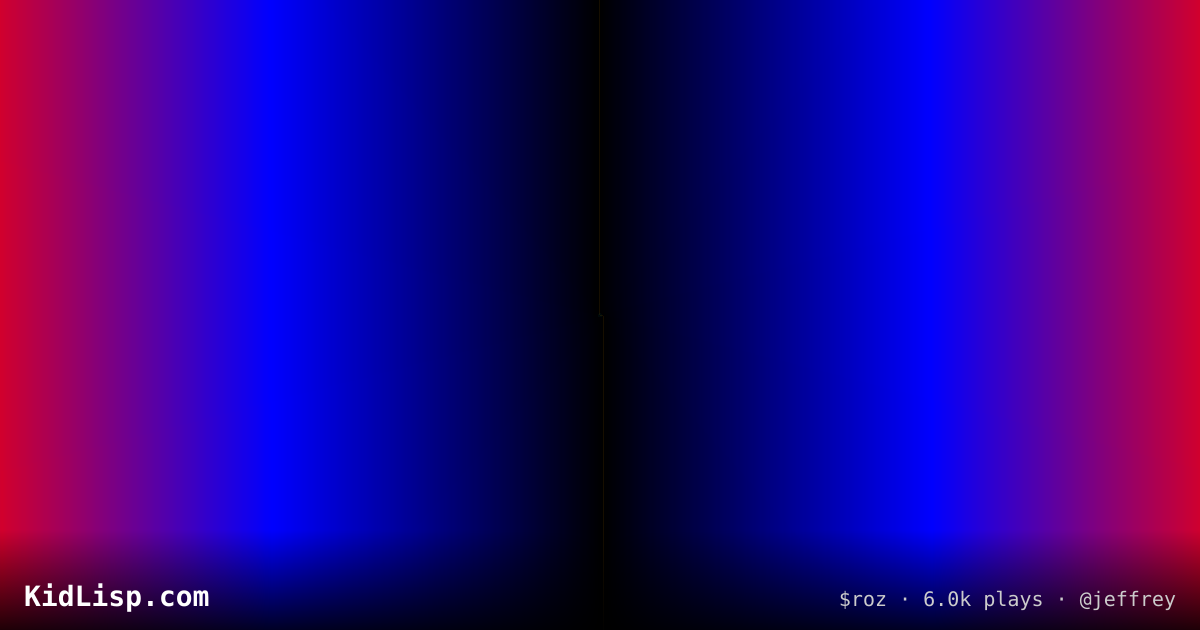
\includegraphics[width=\columnwidth]{kidlisp-og-mosaic.png}
\caption{ovenサービスによってレンダリングされた精選\kidlisp{}プログラム（\texttt{\$roz}）のOpen Graphソーシャルプレビュー。オーバーレイにプログラムコード、再生回数、著者IDが表示される。}
\label{fig:og}
\end{figure}

\section{言語設計}
\label{sec:design}

\kidlisp{}はS式言語である。各プログラムは上から下に評価される式のシーケンスであり、HTML Canvas 2Dコンテキスト、WebGLコンテキスト、Web Audioグラフ、またはそれらの組み合わせに副作用を生む。

\subsection{設計原則}

\begin{enumerate}
  \item \textbf{すべての式が描画する。}有効な\kidlisp{}は可視的な出力を生む。\texttt{main}なし、importなし、ボイラープレートなし。
  \item \textbf{フラットはネストに勝る。}プログラムは抽象の定義ではなく他のプログラムの埋め込みを通じて合成される。これによりコードが一目で読める。
  \item \textbf{構造による安全。}ファイルI/Oなし、ネットワークなし、外部状態の変更なし。プログラムは言語に危険なプリミティブが\emph{ない}ことによってサンドボックス化される。
  \item \textbf{デフォルトでソーシャル。}すべてのプログラムにショートコードとURLがある。共有は配信メカニズムであり、後付けの機能ではない。
\end{enumerate}

\subsection{関数の分類}

118の組み込み関数は12のカテゴリに分類される（表~\ref{tab:functions}）。

\begin{table}[h]
\small
\centering
\begin{tabularx}{\columnwidth}{lrX}
\toprule
\textbf{カテゴリ} & \textbf{数} & \textbf{例} \\
\midrule
グラフィクス & 9 & \texttt{wipe}, \texttt{ink}, \texttt{line}, \texttt{box}, \texttt{circle} \\
変換 & 11 & \texttt{scroll}, \texttt{zoom}, \texttt{spin}, \texttt{blur}, \texttt{suck} \\
数学 & 14 & \texttt{+}, \texttt{sin}, \texttt{cos}, \texttt{random}, \texttt{wiggle} \\
色 & 19 & CSS名 + \texttt{rainbow}, \texttt{zebra} \\
システム & 9 & \texttt{width}, \texttt{height}, \texttt{frame}, \texttt{fps} \\
3D & 8 & \texttt{cube}, \texttt{form}, \texttt{trans}, \texttt{move} \\
オーディオ & 6 & \texttt{mic}, \texttt{melody}, \texttt{overtone} \\
制御 & 7 & \texttt{def}, \texttt{if}, \texttt{repeat}, \texttt{once}, \texttt{later} \\
テキスト & 4 & \texttt{write}, \texttt{type}, \texttt{paste} \\
入力 & 3 & \texttt{pen}, \texttt{touch} \\
合成 & 4 & \texttt{embed}, \texttt{layer}, \texttt{fade} \\
データ & 4 & \texttt{let}, \texttt{list}, \texttt{get}, \texttt{set} \\
\midrule
\textbf{合計} & \textbf{118} & \\
\bottomrule
\end{tabularx}
\caption{カテゴリ別の組み込み関数。}
\label{tab:functions}
\end{table}

\begin{figure}[t]
\centering
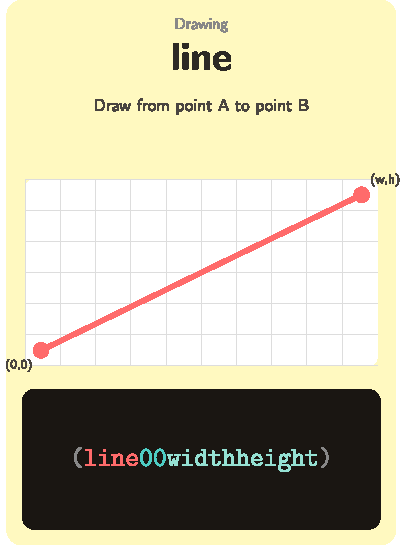
\includegraphics[height=4.5cm]{card-line.pdf}%
\hfill%
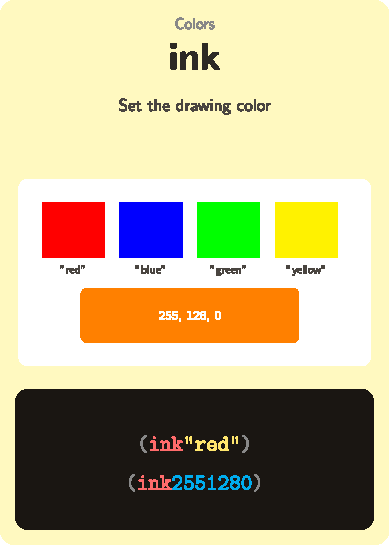
\includegraphics[height=4.5cm]{card-ink.pdf}
\caption{\kidlisp{}の\texttt{line}と\texttt{ink}関数のリファレンスカード。構文と座標出力を表示。カードは\texttt{kidlisp.com/cards}でSVGイラストとして配布。}
\label{fig:cards}
\end{figure}

\subsection{時間構文}

\kidlisp{}は明示的なループやコールバックなしに式の評価をスケジュールする時間演算子を提供する：

\begin{lstlisting}
|\kt{2.5s}| (wipe |\kt{red}|)           ; 2.5秒後
|\kt{1s...}| (spin |\kn{5}|)            ; 毎秒繰り返し
|\kt{3s!}| (write "Done" |\kn{10}| |\kn{10}|)  ; 3秒時に1回だけ実行
|\kt{30f}| (ink |\kt{blue}|)             ; 30フレーム後
\end{lstlisting}

接尾辞\texttt{s}は秒、\texttt{f}はフレーム、\texttt{...}は繰り返し、\texttt{!}は1回実行を示す。これらの演算子は組み合わせ可能：\texttt{0.5s... (ink (random 255) (random 255) (random 255))}は0.5秒ごとに色変化を生む。

\subsection{KidLispが省略するもの}

言語はユーザー定義関数（値の命名用\texttt{def}を除く）、再帰、文字列操作、ファイルI/O、ネットワーク、ミュータブルデータ構造、例外処理を意図的に排除している。これらの省略こそが設計そのものである。抽象化メカニズムを除去することで、プログラムはフラットで読みやすく保たれる——読者はコールスタックを追わずに任意のプログラムを上から下まで理解できる。

\section{エバリュエーターアーキテクチャ}
\label{sec:architecture}

エバリュエーター（\texttt{kidlisp.mjs}、15,161行）は単一のJavaScript ESモジュールであり、ツリー走査インタープリターを実装する。

\subsection{評価モデル}

エバリュエーターはアニメーションフレームごとに1回実行される。S式はトークン化され、ネストされた配列ASTにパースされ、各リストの最初のシンボルへのディスパッチを通じて走査される。組み込み関数はCanvas 2D操作、WebGLコマンド、Web Audio API呼び出し、数学計算に直接マッピングされる。プログラム全体がフレームごとに再評価され、\texttt{frame}と\texttt{time}バインディングが自動更新される——明示的なアニメーションループを不要にする即時モードモデルである。

\subsection{決定論的レンダリング}

同じランダムシードとフレーム番号が与えられれば、プログラムは常に同じ出力を生む。\texttt{random}関数はプログラムのショートコードから初期化されたシードPRNGを使用し、再現可能なジェネラティブアートを実現する。

\subsection{カオスモード}

無効またはランダムなテキスト入力はエラーメッセージではなく芸術的な視覚出力を生成する。信頼度スコアベースの検出器が単語認識率（既知語彙の$<$30\%）、特殊文字比率（$>$50\%）、括弧バランス（比率$>$3:1）をチェックし、入力をコードまたはカオスに分類する。カオス入力は入力テキストからシードされた決定論的なジェネラティブビジュアルを生む。つまり\kidlisp{}に入力された\emph{あらゆる}テキストが視覚コンテンツを生む——ユーザーはエラー状態を一切見ない。

\subsection{パフォーマンス}

エバリュエーターは3段階の最適化を実装する：

\begin{itemize}
  \item \textbf{多段コードキャッシュ}：埋め込みプログラムの解決はRAM、IndexedDB、ネットワーク、次にTEIA（分散型アーカイブ）の順で確認する。キャッシュヒットにより再パースと再取得を回避。
  \item \textbf{バッファプーリング}：解像度ごとに最大8つの再利用可能なオフスクリーンキャンバスで、合成中のアロケーションジッターを回避。
  \item \textbf{自動密度スケーリング}：ピクセル密度をスクロールFPS平均（目標：30--55 FPS）に基づいて0.5xから4xの間で調整し、60フレームのクールダウン期間を設ける。
\end{itemize}

関数呼び出し結果、アルファ調整済みピクセルバッファ、ブレンド合成体はフレームごとにキャッシュおよび無効化される。

\section{ストレージと配信}
\label{sec:infrastructure}

\subsection{MongoDBストレージ}

各プログラムは\texttt{kidlisp} MongoDBコレクション内のドキュメントとして保存される：

\begin{lstlisting}[language=json]
{
  "code": "cow",
  "source": "(wipe blue)\n(ink yellow)...",
  "hash": "a3f2e8...",
  "when": "2025-06-15T...",
  "lastAccessed": "2026-03-01T...",
  "hits": 342,
  "user": "auth0|abc123"
}
\end{lstlisting}

\texttt{hash}フィールド（トリム済みソースのSHA-256）はコンテンツベースの重複排除を強制する：同一のプログラムは常に同一のコードに解決される。\texttt{hits}カウンターと\texttt{lastAccessed}タイムスタンプは利用分析に使用される。コレクションは\texttt{code}と\texttt{hash}のユニークインデックスに加え、\texttt{user}とオプションのNFTミントレコード（\texttt{kept.network}）のスパースインデックスを維持する。

\subsection{コード生成}

ショートコードはソース感知アルゴリズムによって生成される。システムはまずプログラム内容から意味のあるコードの導出を試みる——主要な関数名、色キーワード、構造パターンの抽出——推定されたコードがすべて使用済みの場合はランダム\texttt{nanoid}生成にフォールバックする。これにより\texttt{cow}（牛の形を持つプログラム）のようなコードが任意の英数字文字列ではなく生成される。

\subsection{REST API}

ストレージエンドポイント（\texttt{store-kidlisp.mjs}）は単一のURLで5つのクエリモードを提供する：

\begin{enumerate}
  \item \textbf{POST} --- プログラムの保存。SHA-256ハッシュによる重複排除、ショートコード生成、オプションでATProto（Bluesky）への同期とアーカイブイベントの発行。
  \item \textbf{GET \texttt{?code=xyz}} --- 単一プログラムの取得。\texttt{@handles}コレクションへの\texttt{\$lookup}により著者IDを解決。
  \item \textbf{GET \texttt{?codes=a,b,c}} --- バッチ取得（最大50コード）。評価中の埋め込みレイヤー解決に使用。
  \item \textbf{GET \texttt{?recent=true}} --- 作成日時またはヒット数でソートされたページネーション付きフィード。オプションの\texttt{handle}フィルターでユーザー別フィード。
  \item \textbf{GET \texttt{?stats=functions}} --- コーパス横断の関数使用分析。プログラム人気度で重み付けされたカウントを返す。
\end{enumerate}

認証はオプションで3秒タイムアウト——匿名プログラム作成をサポートするが、認証済みユーザーは帰属とアーカイブイベント発行を得る。

\subsection{埋め込みと合成}

プログラム内の\texttt{\$code}構文はストレージAPIからの取得（またはキャッシュヒット）、オフスクリーンバッファでの評価、親キャンバスへの合成をトリガーする。これにより有向非巡回合成グラフが生まれる。実例：

\begin{lstlisting}
; A 3D grid of cubes with embedded layers
(wipe |\kt{black}|)
(def |\kv{gridsize}| |\kn{6}|)
(repeat (|\km{*}| |\kv{gridsize}| |\kv{gridsize}|) |\kv{i}|
  (ink (hop |\kn{0.1}| |\kt{rainbow}| |\kt{blue}| |\kt{white}|))
  (form (trans (cube |\kv{i}|)
    (move (|\km{*}| (|\km{\%}| |\kv{i}| |\kv{gridsize}|) |\kn{3}|) |\kn{0}| |\kn{-20}|)
    (scale |\kn{1.5}|) (spin |\kn{0}| |\kn{1}| |\kn{0}|))))
(|\ke{\$27z}|)
(|\ke{\$cow}|)
\end{lstlisting}

ここで\texttt{\$27z}と\texttt{\$cow}はMongoDBから解決され、オフスクリーンバッファにレンダリングされ、合成される。ユーザーは複雑な単一プログラムを書く代わりに、単純なプログラムを重ね合わせて複雑なビジュアルを構築する。

\section{メディアパイプライン}
\label{sec:media}

ovenサービス（\texttt{oven.aesthetic.computer}）は録画された\kidlisp{}セッションを共有可能なメディアアセットに変換する。

\subsection{録画からMP4へ}

ユーザーがセッションを録画すると、セッションサーバーがPNGフレームとオプションのWAVオーディオを含むZIPをアップロードする。oven：

\begin{enumerate}
  \item フレームを抽出し\texttt{timing.json}から各フレーム持続時間を読み取る
  \item 中間フレームからサムネイルを生成（3倍最近傍拡大、512$\times$512にフィット）
  \item FFmpegを通じて最近傍拡大でH.264/AAC MP4にエンコードし、ピクセルアート美学を保持
  \item DigitalOcean Spaces CDNにアップロード
  \item \texttt{oven-bakes} MongoDBコレクションにベイクメタデータを保存し、WebSocketを通じてサブスクライバーに通知
\end{enumerate}

ovenは\texttt{tapes} MongoDBコレクションをchange streamsで監視し、処理が必要な新しい録画を自動検出する。

\begin{figure}[t]
\centering
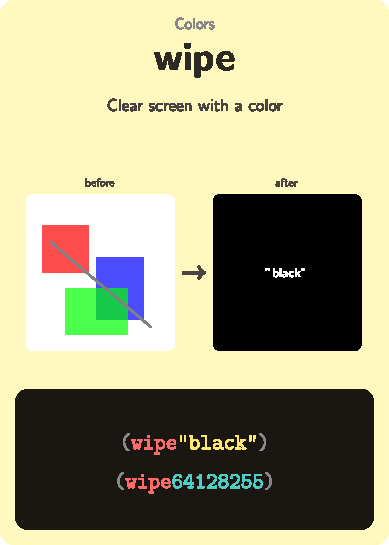
\includegraphics[height=4.5cm]{card-wipe.pdf}%
\hfill%
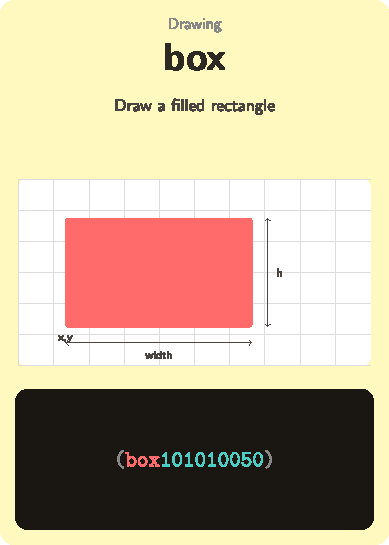
\includegraphics[height=4.5cm]{card-box.pdf}
\caption{\texttt{wipe}（色で画面をクリア）と\texttt{box}（矩形を描画）のリファレンスカード。各カードに関数シグネチャ、グリッド上のビジュアル例、対応するソースコードを表示。}
\label{fig:cards2}
\end{figure}

\subsection{ソーシャルプレビュー画像}

ovenはソーシャル共有用に安定したURL（例：\texttt{/kidlisp-og.png}）のOpen Graphプレビュー画像を生成する。iOSクローラーは直接の画像配信を要求し——\texttt{og:image} URLの301リダイレクトをフォローしない——ためovenは生成済みPNGをキャッシュして即時200レスポンスで配信し、キャッシュミス時に非同期再生成をトリガーする。

\subsection{アセット配信}

すべてのメディアアセットはDigitalOcean Spaces CDN（\texttt{art-aesthetic-computer.sfo3.cdn.\allowbreak digitaloceanspaces.com}）を通じて配信される。録画テープは独立したバケット（\texttt{at-blobs-aesthetic-computer}）とオプションのカスタムCDNドメインを使用する。Netlifyが\texttt{/preview/*}と\texttt{/icon/*}パスをovenにプロキシし、透過的なURL解決を実現する。

\section{開発環境}

\kidlisp{} IDEは\texttt{kidlisp.com}に位置し、Monacoベースのエディタ（カスタム構文ハイライト付き）、Aesthetic Computerランタイムを実行するライブプレビューiframe、コンソールパネル、再生コントロール（再生/一時停止/停止）を提供する。

「スライダーモード」ではエディタ内の数値リテラルをドラッグして値をリアルタイムに調整できる——カーソルが任意の数値上で水平スライダーに変わり、ドラッグ中もプレビューが継続更新される。

IDEは2つのレイアウトモードをサポートする：\emph{スタジオ}（分割画面のエディタ、プレビュー、コンソール）と\emph{ステージ}（エディタがフルスクリーンキャンバスに直接オーバーレイし、透明背景で、すべてのUI要素が非表示）。ステージモードはライブパフォーマンスシナリオ向けに設計されており、コード自体が視覚出力の一部となる。

\section{開発史}
\label{sec:history}

以下のタイムラインはAesthetic Computerリポジトリのgit履歴から再構成された（2024年4月から2026年3月の間に\texttt{kidlisp.mjs}に触れた626コミット）。

\subsection{フェーズ1：プロトタイプ（2024年4--6月）}

開発は2024年4月17日、「mock lisp」というコミットタイトルで始まった。3日以内にS式パーサーが動作し、\texttt{ink}と\texttt{line}が数値引数を受け入れ、プログラムをACプロンプトに直接入力できるようになった。4月末に変数定義用の\texttt{def}が追加された。2024年5月と6月の計66コミットで、コア描画関数、\texttt{later}時間構造、1回実行用の\texttt{once}、プログラムの匿名公開が追加された。エバリュエーターは約1,000行に達した。

\subsection{フェーズ2：停滞（2024年7月--2025年5月）}

11か月間、\texttt{kidlisp.mjs}に触れるコミットはなかった。言語はACプロンプトに埋め込まれた利用可能なプロトタイプとして存在したが、ストレージバックエンド、埋め込み、オーディオ、専用エディタを欠いていた。

\subsection{フェーズ3：急速拡張（2025年6--8月）}

開発は2025年6月に再開し、月間82コミット。エバリュエーターは1,760行から8月には4,965行に成長した。主な追加：

\begin{itemize}
  \item \textbf{2025年6月}：メロディーパーサー、クロック構文、フレームごとのレンダリングモデル、テストスイート（\texttt{kidlisp-spec.js}）。
  \item \textbf{2025年7月}：MongoDBストレージバックエンド（\texttt{store-kidlisp.mjs}）、ショートコード生成、QRコード共有、録画とGIFエクスポート、マイク入力（\texttt{mic}）とフォールバックアニメーション。
  \item \textbf{2025年8月}：埋め込みレイヤー（\texttt{\$code}構文）とアルファ合成・オフスクリーンバッファ、プログラムをNFTとしてミントするTezosブロックチェーン統合、\texttt{fade}グラデーションとピクセルバッファ最適化。
\end{itemize}

エバリュエーターは2025年9月末に10,000行を超えた。

\subsection{フェーズ4：プラットフォーム統合（2025年9--12月）}

10月だけで108コミット（ピーク月）。このフェーズで\kidlisp{}はより広いAesthetic Computerエコシステムに統合された：

\begin{itemize}
  \item \textbf{2025年9月}：レイヤー0アーキテクチャ（消去モード）、MP4エクスポート用のベイク層、パフォーマンスクリティカルな埋め込みレイヤー修正。
  \item \textbf{2025年10月}：ATProto/Bluesky連合（プログラムがソーシャルメディア投稿として連合配信）、クロスプラットフォームバンドル用のPACKモード、リアルタイム数値パラメータ調整用のスライダーモード。
  \item \textbf{2025年11月}：\texttt{kidlisp.com} IDEがローンチ（Monacoエディタ、ライブプレビュー、コンソール、再生コントロール）、デバッグ用の実行トレースシステム、NFTワークフローが「OBJKT」から「keep」にリネーム。
  \item \textbf{2025年12月}：リファレンスカード（各関数のSVGイラスト）、NFT用IPFSサムネイル生成、ソーシャル共有用のoven OG画像生成、自動密度パフォーマンススケーリング。
\end{itemize}

\subsection{フェーズ5：洗練（2026年1--3月）}

エバリュエーターは15,161行で安定。新規追加にはカオスモード（2026年2月）、3Dプリミティブ（\texttt{cube}、\texttt{form}、\texttt{trans}）、バンドオーディオ変数、\texttt{flip}コマンド、ライブパフォーマンス用ステージモードが含まれる。開発は機能追加からロバスト性に移行：埋め込みレイヤーのパフォーマンス退行の修正、カオスモードの誤分類防止、キャッシュ無効化の改善。

\begin{table}[h]
\small
\centering
\begin{tabular}{lrl}
\toprule
\textbf{日付} & \textbf{行数} & \textbf{マイルストーン} \\
\midrule
2024年4月 & 0 & 初回コミット（「mock lisp」） \\
2024年6月 & $\sim$1{,}000 & コア描画、時間、変数 \\
2025年6月 & 1{,}760 & 開発再開 \\
2025年8月 & 4{,}965 & 埋め込み、オーディオ、ストレージ \\
2025年9月 & 10{,}382 & レイヤーアーキテクチャ、ベイク \\
2025年12月 & 13{,}877 & IDE、カード、OG画像 \\
2026年2月 & 15{,}161 & カオスモード、3D、洗練 \\
\bottomrule
\end{tabular}
\caption{エバリュエーターの行数成長（\texttt{kidlisp.mjs}）。}
\label{tab:growth}
\end{table}

\section{評価}
\label{sec:evaluation}

2026年3月時点の採用指標を表~\ref{tab:adoption}に示す。

\begin{table}[h]
\small
\centering
\begin{tabular}{lr}
\toprule
\textbf{指標} & \textbf{値} \\
\midrule
作成されたプログラム総数 & 16,174 \\
個別著者数 & 59 \\
著者あたりプログラム数（中央値） & 12 \\
著者あたりプログラム数（第3四分位） & 180+ \\
埋め込み深度（観測最大値） & 7層 \\
プラットフォーム登録ユーザー & 2,798 \\
\bottomrule
\end{tabular}
\caption{採用指標（2026年3月）。}
\label{tab:adoption}
\end{table}

\subsection{関数使用分析}

\texttt{?stats=functions} APIエンドポイントはコーパス横断の重み付き関数使用カウントを提供する。最大5,000プログラム（ヒット数順）をスキャンし、各ソースを解析して関数呼び出しを抽出し、プログラム人気度で重み付けされたカウントを返す。これによりユーザーが好むプリミティブの定量分析が可能となる。最も使用頻度の高い関数は\texttt{wipe}、\texttt{ink}、\texttt{repeat}、\texttt{circle}——ユーザーが主に描画とイテレーションを使用していることを確認する。

\subsection{観察}

\textbf{抽象より合成。}ユーザーは抽象化ではなく埋め込みを行う。最も参照されるプログラムは単純なビジュアルプリミティブ（グラデーション、形状、パターン）であり、ビルディングブロックとして機能する。

\textbf{エンジニアリングより探索。}プログラムは通常短い（10行以下）。ユーザーは既存プログラムを編集するのではなく新しいプログラムを保存してイテレーションし、ストレージタイムスタンプに可視的な分岐探索パスを作り出す。

\textbf{ソーシャル学習。}最も生産性の高い著者は既存プログラムの閲覧とリミックスから始める。ショートコードシステムにより発見は偶発的になる——ユーザーはランダムなコードを試すことでプログラムに出会う。

\subsection{制約}

\kidlisp{}は汎用プログラミング、複雑なシミュレーション、セッション間で持続的な状態を必要とするアプリケーションには適さない。ユーザー定義関数の欠如はプログラムの複雑さを制限する——これは意図的な選択だが、一部の上級ユーザーはこれにフラストレーションを感じる。

\section{関連研究}

\textbf{クリエイティブ・プログラミング。}Processing~\citep{reas2007processing}とp5.js~\citep{mccarthy2015p5js}が主流ツールである。openFrameworksはC++を使用する。いずれもプロジェクト構造の管理と汎用プログラミング言語の理解を必要とする。

\textbf{ライブコーディング。}Hydra~\citep{hydra2019}はJavaScriptメソッドチェーンを使用するブラウザベースのライブビジュアルプログラミングを提供するが、永続ストレージやソーシャル機能を持たない。Sonic Pi~\citep{aaron2016sonic}は音楽教育を対象とする。Fluxus~\citep{fluxus2007}はSchemeで3Dビジュアルを行うが、もはやメンテナンスされていない。

\textbf{教育言語。}Scratch~\citep{resnick2009scratch}はソーシャル共有が教育プログラミングの参加を促進することを証明した。\kidlisp{}はこの知見を継承しつつ、テキストベースのLisp構文を使用し、汎用教育ではなくジェネラティブアートを対象とする。

\textbf{アート用Lisp。}Racketの\texttt{2htdp/image}ライブラリ~\citep{racket2018}はCS教育のための関数型画像構築を提供するが、ソーシャル配信を伴うリアルタイムアニメーションではなく、静的画像と教育法を対象としている。

\section{結論}

\kidlisp{}は、ミニマルなドメイン固有言語——ブラウザネイティブで、ユーザー定義の抽象なし、ソーシャル配信を備えたコンテンツアドレスドデータベースに支えられた——がジェネラティブアート実践の活発なコミュニティを支えうることを実証する。核心的な設計上の知見は、ソーシャル配信（ショートコード、URL共有、埋め込み）が付加機能ではなくコア言語機能であり、ユーザーがどう学び、創り、互いの作品の上に構築するかを形作るということである。

埋め込みグラフ、関数使用分析API、そしてタイムスタンプと著者帰属を持つ16,000以上のプログラムコーパスは、クリエイティブ・プログラミング実践、計算的創造性、非専門家ユーザーがソーシャルな関与を通じて関数型プログラミングをどう学ぶかを研究するためのデータセットを構成する。

\kidlisp{}はISCライセンスの下でオープンソースである。エバリュエーター、ドキュメント、ツールは\url{https://github.com/digitpain/aesthetic.computer}で入手可能。プログラムは\url{https://kidlisp.com}で閲覧・作成できる。

\vspace{0.5em}
\noindent\textit{英語原版からの翻訳。原版は \url{https://papers.aesthetic.computer} にて入手可能}

\vspace{0.5em}
\noindent\textbf{ORCID:} \href{https://orcid.org/0009-0007-4460-4913}{0009-0007-4460-4913}

\bibliographystyle{plainnat}
\bibliography{references}

\end{document}
